%Arquivo contendo o capítulo Revisão Bibliográfica
\chapter{Revisão Bibliográfica} \label{cap:revbib}
Este capítulo tem como objetivo descrever os principais conceitos apresentados para o desenvolvimento do Pedal-to-Play. Os conceitos envolvidos são: jogo pervasivo; gamificação; desenvolvimento multiplataforma; aplicativos de saúde e \textit{fitness}; avatares virtuais e geolocalização.

\section{Jogos Pervasivos}
Um jogo pervasivo é um tipo de jogo digital, no qual ao menos uma interação do usuário com o sistema transcorre no universo físico. Eles integram os aspectos físicos e sociais do mundo real em jogos digitais, estendendo a interação do jogador com o jogo, pois em ambientes virtuais a interface com o usuário está limitada ao uso dos periféricos do computador. Os recentes dispositivos celulares (\textit{smartphones}) e a popularização de tecnologias de rede sem fio 
(tais como, \textit{WiFi\footnote{WiFi é o termo popular para redes sem fio \textit{ethernet} padrão  WLANs (Wireline Local Area Networks) \cite{lehr2003}.} e 3G\footnote{3G refere-se à terceira geração de serviços de dados móveis, fornecido por operadoras provedoras de redes móveis \cite{lehr2003}.}}) facilitam a extensão das interfaces homem-computador \cite{magerkurth2005, vianna2013}. Um exemplo de jogo pervasivo é o Human Pacman. \par

\begin{figure}[h]
    \caption[Processo de coleta de um item no Human Pacman]{Processo de coleta de um item no Human Pacman \cite{cheok2003}.}
    \centerline{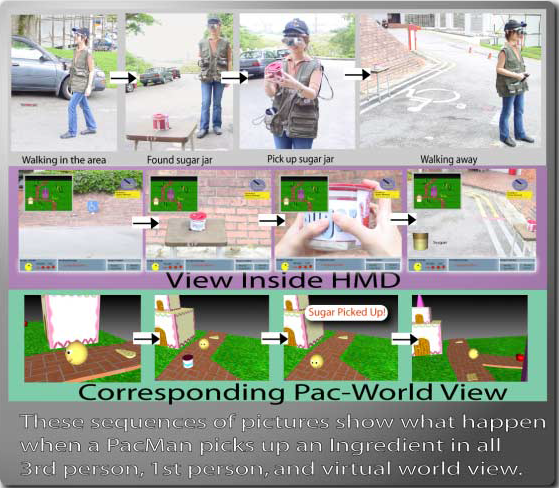
\includegraphics[width=20em]{figuras/humanpacman.png}}
    \label{fig:humanpacman}
\end{figure}

No Human Pacman, os jogadores interpretam o papel dos personagens do jogo Pac-Man no mundo real, enquanto vestem-se com trajes customizados integrados a dispositivos eletrônicos. Esses trajes permitem interação entre os jogadores via WiFi e interação com o sistema que insere elementos virtuais no mundo físico, através de técnicas de realidade aumentada, como ilustrado na Figura \ref{fig:humanpacman} \cite{cheok2003}. 

\section{Gamificação}
A gamificação (do original em inglês \textit{gamification}) consiste na aplicação de mecanismos de jogos com o intuito de resolver problemas práticos ou motivar um público específico a realizar certas atividades em contextos fora de jogos. Alguns exemplos de aplicação de gamificação têm como objetivo: agilizar processos de aprendizagem ou treinamento; tornar mais agradáveis tarefas consideradas tediosas ou repetitivas; motivar usuários a reforçar a condição física e emocional e até usar jogos em forma de propagandas de produtos e serviços. O Duolingo\footnote{\url{https://www.duolingo.com/}} é um exemplo de \textit{software} "gamificado" para agilizar processos de aprendizagem de uma língua estrangeira e o SuperBetter\footnote{\url{https://www.superbetter.com/}}, para incentivar o usuário a reforçar o condicionamento físico. \cite{vianna2013, zichermann2011}.

\section{Desenvolvimento Multiplataforma}
Com a intenção de garantir que o \textit{software} possua portabilidade para plataformas \textit{mobile} e \textit{desktop} se fará uso do desenvolvimento Web. Segundo \citet{lopes2013}, o desenvolvimento Web é democrático, aberto e acessível, pois praticamente, todo dispositivo possui um navegador (\textit{web browser}). Uma aplicação Web garante acesso a um número maior de usuários do que uma aplicação nativa para um determinado dispositivo. Lopes também salienta que é cada vez mais comum usar as linguagens fundamentais da Web para desenvolver aplicativos \textit{mobile}. A subseção seguinte versará sobre as tecnologias fundamentais do desenvolvimento Web.

\subsection{Lado do Cliente}
As tecnologias fundamentais usadas em sistemas Web, no lado do cliente, são o \textit{Hyper Text Markup Language} (HTML), o \textit{Cascading Style Sheets} (CSS) e o JavaScript (JS). \par

HTML5 é a versão atual do HTML, linguagem de marcação para escrever a estrutura principal de páginas Web. HTML fornece instruções aos \textit{web browsers} (exemplos: Chrome, Internet Explorer, Firefox) sobre o que exibir em uma página. Cada conteúdo é representado por um conjunto de elementos pré-definidos chamados \textit{tags} \cite{html5}. \par 

CSS é a linguagem usada para definir o estilo e o \textit{layout} do conteúdo de uma página HTML. Ela também permite ajustar o \textit{layout} das aplicações para qualquer tamanho de tela, inclusive o \textit{mobile}. Esta característica é importante para o \textit{software} deste trabalho, o qual deve ser multiplataforma. A versão atual do CSS é o CSS3 \cite{css3}. \par
 
JS é uma linguagem de programação interpretada e orientada a objetos, usada para manipular o comportamento de páginas HTML. Possui recursos para alterar o conteúdo das páginas, o estilo delas e validar entradas do usuário \cite{javascript}. \par

No desenvolvimento do lado do cliente também podem ser empregados \textit{frameworks} e bibliotecas. Estes se propõem a facilitar o uso das linguagens listadas anteriormente, assegurar questões de compatibilidade entre navegadores, assegurar questões de segurança e confiabilidade e de portabilidade para diferentes dispositivos. \par

Os seguintes \textit{frameworks} foram utilizados no desenvolvimento do \textit{software}: Bootstrap\footnote{\url{http://getbootstrap.com/}}, para desenvolvimento de páginas Web responsivas e adaptáveis para dispositivos com tamanhos diversos; AngularJS\footnote{\url{https://angularjs.org/}}, \textit{frameworks} de JS usado para tornar páginas HTML estáticas em páginas dinâmicas, estendendo o vocabulário do HTML e propondo um modelo de projeto modularizado e jQuery\footnote{\url{https://jquery.com/}}, usado para facilitar e estender a capacidade do JS de manipulação do DOM\footnote{Document Object Model é uma interface que permite aos programas e \textit{scripts} alterarem de forma dinâmica as propriedades de uma página Web. \cite{w3cDOM}}. \par
 
A plataforma Cordova\footnote{\url{https://cordova.apache.org/}}, para desenvolvimento de aplicativos multiplataforma, também foi utilizada. Ela permite  converter sistemas Web em aplicações nativas \textit{mobile} e atribui ao \textit{software} acesso aos recursos de \textit{hardware} dos dispositivos \textit{mobile}. 

\subsection{Lado do Servidor} \label{sec:server}
Atualmente o pódio das tecnologias para o desenvolvimento Web do lado do Servidor está ocupado pelo PHP, em primeiro lugar; ASP.NET em segundo e o Java, em terceiro \cite{w3techs2015}. \par

Java Web consiste na implementação das APIs de Servlets e JavaServer Pages (JSP). Servlet é a tecnologia usada pelo Java para geração de páginas HTML dinâmicas, são classes Java com HTML embutido. Páginas JSP consistem no inverso, são estruturadas como páginas HTML com código Java embutido. Servlets e JSP podem ser desenvolvidos na plataforma Java Enterprise Edition (Java EE). A Java EE consiste em um conjunto de especificações para várias APIs de desenvolvimento Java para Web \cite{basham2008}. Os pontos fortes do Java Web estão na portabilidade para diferentes plataformas de \textit{hardware}, banco de dados e servidores e a grande quantidade de \textit{frameworks} existentes, tais como Primefaces\footnote{\url{http://www.primefaces.org/}} e Spring\footnote{\url{http://spring.io/}}. \par

ASP.NET é uma tecnologia da Microsoft, parte do .NET \textit{Framework} para desenvolvimento de aplicações Web. O desenvolvimento com ASP.NET pode ser feito com qualquer linguagem compatível com o .NET. Algumas das vantagens desta tecnologia envolvem a separação clara entre a interface do usuário e a lógica de programação; a familiaridade com o desenvolvimento \textit{desktop}; a ferramenta de desenvolvimento Visual Studio, com diversos recursos para facilitar o trabalho do desenvolvedor e a integração com todos os recursos do \textit{framework} .NET \cite{imar2014}. As desvantagens do ASP.NET são: sua limitação ao sistema operacional Windows e a licença de uso profissional do Visual Studio não ser gratuita. \par

PHP é uma linguagem de programação presente em 10 milhões de sites no mundo inteiro. O PHP adiciona dinamismo às páginas estáticas e automatiza tarefas, diminuindo mão-de-obra. Possui portabilidade para várias plataformas \textit{desktop} (exemplos: Linux, Unix e Windows); possui código aberto e licença de uso gratuita; suporta vários bancos de dados (entre eles: MySQL, Oracle e PostgreSQL) \cite{niederauer2004, welling2003}. \par

Outros pontos fortes do PHP envolvem sua alta performance (um único servidor pode lidar com milhões de acessos por dia); bibliotecas nativas para várias tarefas comuns na Web (funções para gerenciamento de imagens, conexão com \textit{web services}, interpretação de XML, envio de \textit{email}, gerenciamento de \textit{cookies} e geração de documentos PDF); fácil aprendizado (a sintaxe de PHP é baseada em outras linguagens, entre elas, C e Perl); suporte ao desenvolvimento orientado a objetos e disponibilidade de suporte técnico \cite{welling2003}. \par

Decidiu-se usar a linguagem PHP para desenvolvimento do lado do servidor, pois comparado com as outras duas principais linguagens (ASP.NET e Java) o PHP se destaca por sua licença gratuita, portabilidade e suporte nativo (sem \textit{frameworks}) a funcionalidades que serão essenciais no software deste trabalho, tais como: gerenciamento de imagens, interpretação de arquivos JSON e acesso a banco de dados. \par

O servidor disponibiliza um serviço Web (\textit{web service}) para a aplicação cliente. \textit{Web services} são soluções para integração entre aplicações diferentes. As duas arquiteturas mais utilizados para o desenvolvimento de \textit{web services} são o SOAP e o REST. 

\par A arquitetura SOAP (Simple Object Access Protocol) define padrões para integração e troca de informação entre sistemas descentralizados baseando-se na transferências de arquivos no formato XML (eXtensible Markup Language). A SOAP também engloba um conjunto de especificações, atualmente mantidas pela W3C (World Wide Web Consortium) \citeyearpar{w3cSOAP}.

\par A arquitetura REST (Representational State Transfer) foi proposta pela primeira vez por Roy Fielding (um dos membros fundadores da Apache\footnote{http://www.apache.org/} e do protocolo HTTP), em sua tese de doutorado \citeyearpar{fielding2000} . Fielding especificou esta arquitetura pelas seguintes propriedades: 

\begin{itemize}
\item Modelo Cliente-Servidor: característica comum de aplicações Web, na qual o cliente requisita um recurso para um servidor e este encaminha de volta uma resposta de sucesso ou erro;

\item Ausência de estado: cada requisição ao servidor deve conter toda informação necessária para seu processamento. Por exemplo, o servidor não mantém sessões de usuários;

\item \textit{Cache}: permite que respostas definidas como \textit{cacheable} sejam reutilizadas para futuras requisições equivalentes; 

\item Interface uniforme: característica central do REST, na qual os recursos são identificados e manipulados por representações, as mensagens são auto descritivas e a hipermídia\footnote{Hipermídia refere-se a um conjunto de arquivos existentes no meio digital. \cite{dictionary2011hypermedia}} define o estado da aplicação;

\item Multicamada: permite a disposição de diferentes funcionalidades em diferentes camadas do sistema; 

\item \textit{Code-On-Demand}: característica opcional que possibilita que os clientes baixem e executem a funcionalidade diretamente. 
\end{itemize}

Outra característica importante do REST é que a hipermídia transferida entre cliente e servidor não tem formato padrão, diferente do SOAP, o qual permite somente o formato XML.

\par 
Decidiu-se utilizar no servidor do Pedal-to-Play o protocolo de comunicação HTTP e a arquitetura REST, pois os padrões do SOAP engessam em demasia o formato das requisições entre cliente e servidor, as quais se tornam maiores do que as requisições REST (referente à quantidade de \textit{bytes}), tal como Dal Moro et al. \citeyearpar{dal2009web} demonstraram em seu trabalho. Requisições menores consumem menos dados móveis e por este motivo são uma vantagem para o projeto que tem uma versão \textit{mobile}.

\par 
O uso de XML também não é interessante para a aplicação, pois o lado do cliente será desenvolvido com JavaScript, o qual tem seus objetos no padrão JavaScript Object Notation (JSON)\footnote{\url{http://www.json.org/}}. Por consequência, a interpretação de XML seria mais custosa, em termos de processamento e desenvolvimento, do que a de mensagens JSON, qual é nativa da linguagem. 
\par
Por fim, no quesito sistemas de gerenciamento de banco de dados (SGDB), os três mais usados atualmente, segundo o \textit{site} da DB-Engines\citeyearpar{dbEngines2015}, são o Oracle em primeiro lugar, o MySQL em segundo e o Microsoft SQL Server em terceiro. O MySQL possui licença de uso \textit{open source} e versão gratuita sem restrições, enquanto o Oracle e o Microsoft SQL Server são \textit{softwares} com licença de uso comercial. Por estes motivos decidiu-se fazer uso do MySQL, o qual, em conjunto com o PHP, também possui serviços gratuitos de hospedagem \textit{online} como os do Hostinger\footnote{\url{http://www.hostinger.com.br/}} e do OpenShift\footnote{\url{https://www.openshift.com/}}. 

\section{Avatares Virtuais}
Avatares são corpos virtuais criados para representar a identidade e ações de um usuário em um mundo virtual. Eles são usados como ferramentas de comunicação e para representar visualmente os usuários. Uma das principais características dos avatares é a sua customização, orientada pelo desejo de quem o cria \cite{ducheneaut2009}. Um exemplo de aplicativo específico para criação de avatares e utilização destes como ferramenta de socialização entre os usuários é o \textit{BuddyPoke}, ver Figura \ref{fig:avatar}. \par

\begin{figure}[h]
    \caption{Exemplo de avatar criado no aplicativo BuddyPoke.}
    \centerline{
\includegraphics[width=15em]{figuras/avatar.png}}
    \label{fig:avatar}
\end{figure}
\centerline{Fonte: Página oficial do BuddyPoke na Web\footnote{Disponível em: <\url{http://www.buddypoke.com/}>. Acesso em jun. 2015.}}

\section{Aplicativos de Saúde e \textit{Fitness}}
Aplicativos de Saúde e \textit{Fitness} são \textit{softwares} desenvolvidos para dispositivos \textit{mobile} com o objetivo de estimular o usuário a praticar atividades benéficas à saúde e ao bem-estar \cite{bonome2012}. Alguns exemplos dessa categoria de aplicativos são o Strava\footnote{\url{https://www.strava.com/}} e o Runtastic Road Bike\footnote{\url{https://www.runtastic.com/}}.

\par Esses aplicativos fornecem ao usuário a funcionalidade de monitorar suas atividades físicas utilizando os recursos de Geolocalização dos dispositivos móveis. As atividades monitoradas são analisadas e persistidas, de forma que o usuário possa visualizá-las graficamente em outros momentos e acompanhar as estatísticas geradas a partir delas. O monitoramente de atividades também resulta em prêmios virtuais

\par Os aplicativos de saúde e \textit{fitness} também proporcionam funcionalidades para interação social. Permitem aos usuários acompanharem o perfil de outros, a competição por melhores métricas nas pedaladas e também a criação de segmentos, os quais são desafios baseados em trajetos compartilhados por todos os usuários.

\section{Geolocalização}
Geolocalização é o termo usado para descrever o posicionamento geográfico de um objeto no planeta, a partir de seus valores de latitude e longitude \cite{aires2014}. Essas coordenadas podem ser obtidas utilizando diferentes tecnologias. Entre elas temos o \textit{Global Positioning System} (GPS), um sistema desenvolvido e mantido pelas Forças Aéreas dos Estados Unidos. Este sistema consiste em três segmentos: o espacial, composto por 24 satélites operantes em órbita e transmitindo sinais de radio; o controle, o qual consiste nas estações de controle que mantêm os satélites funcionando adequadamente; e o segmento do usuário, o qual compreende os aparelhos receptores dos sinais vindos dos satélites \cite{gpsgov}. O funcionamento do GPS é ilustrado na Figura \ref{fig:gps}. \par

\begin{figure}[h]
    \caption[Funcionamento do GPS]{Funcionamento do GPS \cite{cesani2013}.}
    \centerline{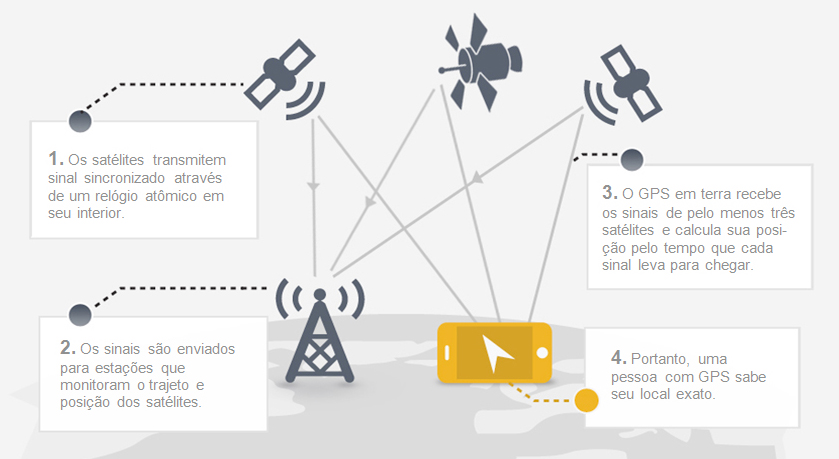
\includegraphics[width=34em]{figuras/gps.png}}
    \label{fig:gps}
\end{figure}

No \ entanto, o uso de GPS tem suas limitações. Segundo \citet{sukaphat2013}, os sinais de GPS possuem um alcance limitado e uma capacidade baixa de atravessar barreiras. Estas características impedem o funcionamento adequado desta tecnologia em ambientes fechados. 

Entre as outras tecnologias de geolocalização está a análise de assinaturas de rede como o endereço IP, RFID, WIFI, endereço de MAC Bluetooth e GSM/CDMA Cell ID (identificadores das antenas das redes de telefonia móvel) \cite{w3cGeo}.
\par

\section{Conclusões}
Neste capítulo foram descritos os principais conceitos que permeiam o projeto. Entre eles, o conceito de \textbf{jogo pervasivo}, no qual o Pedal-to-Play se caracteriza devido a sua funcionalidade de monitoramento da atividade de ciclismo do usuário, através das técnicas de \textbf{geolocalização}. O conceito de \textbf{aplicativo de saúde e \textit{fitness}}, no qual o projeto pode ser categorizado, pois foca em uma atividade desportiva. Também foi versado sobre as tecnologias de \textbf{desenvolvimento Web}, quais atendem ao objetivo do sistema ser multiplataforma e os \textit{frameworks} que foram utilizados, tais como AngularJS e Bootstrap, no lado do cliente; o Cordova para geração do aplicativo \textit{mobile} e o \textit{web service} REST, com PHP e MySQL, para o lado do servidor. E por fim, foram apresentados os conceitos de \textbf{gamificação} e \textbf{avatares virtuais}, quais serão o diferencial do Pedal-to-Play em relação aos demais sistemas já existentes na mesma modalidade, alguns desses sistemas serão apresentados no próximo capítulo.